\section{リリースについて}
最終成果発表会で得られた意見をもとに第4サイクルの改善フェーズを行った後、続く第5サイクルでアプリケーションへ反映させる予定である。リリース時期は2月中を目標としている。この時期にリリースの目標を設定した理由としては、3月に北海道新幹線が開業することが挙げられる。観光客が最も訪れると予想される開業直後に間に合うようリリース準備を進めていく予定である。今後の作業としては、まずレビューの結果をもとに機能の拡張やUIの再設計を行い、並行して既知のバグの修正を行っていく。これらが完了し次第、App Storeへリリースする。また、リリース後にも定期的なメンテナンスを行っていくほか、季節ごとのコンテンツの追加などの案も検討されている。なお、メンテナンスの方法や継続期間についての検討も開発と並行して行っていく予定である。
\begin{figure}[htbp]
  \begin{flushleft}
    \begin{tabular}{c}

      % 1
      \begin{minipage}{0.7\hsize}
        \begin{center}
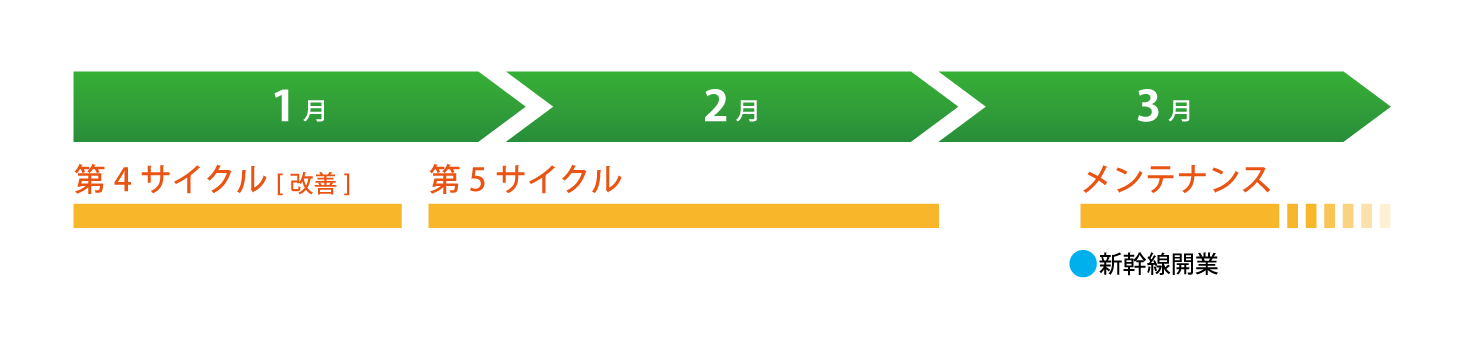
\includegraphics[width=15cm, bb=0 0 1478 338]{release-1.png}
       
        \end{center}
      \end{minipage}

    \end{tabular}
    \caption{今後の予定}
    \label{fig:lena}
  \end{flushleft}
\end{figure}
\bunseki{横山翔栄}